\documentclass{article}[18pt]
\ProvidesPackage{format}
%Page setup
\usepackage[utf8]{inputenc}
\usepackage[margin=0.7in]{geometry}
\usepackage{parselines} 
\usepackage[english]{babel}
\usepackage{fancyhdr}
\usepackage{titlesec}
\hyphenpenalty=10000

\pagestyle{fancy}
\fancyhf{}
\rhead{Sam Robbins}
\rfoot{Page \thepage}

%Characters
\usepackage{amsmath}
\usepackage{amssymb}
\usepackage{gensymb}
\newcommand{\R}{\mathbb{R}}

%Diagrams
\usepackage{pgfplots}
\usepackage{graphicx}
\usepackage{tabularx}
\usepackage{relsize}
\pgfplotsset{width=10cm,compat=1.9}
\usepackage{float}

%Length Setting
\titlespacing\section{0pt}{14pt plus 4pt minus 2pt}{0pt plus 2pt minus 2pt}
\newlength\tindent
\setlength{\tindent}{\parindent}
\setlength{\parindent}{0pt}
\renewcommand{\indent}{\hspace*{\tindent}}

%Programming Font
\usepackage{courier}
\usepackage{listings}
\usepackage{pxfonts}

%Lists
\usepackage{enumerate}
\usepackage{enumitem}

% Networks Macro
\usepackage{tikz}


% Commands for files converted using pandoc
\providecommand{\tightlist}{%
	\setlength{\itemsep}{0pt}\setlength{\parskip}{0pt}}
\usepackage{hyperref}

% Get nice commands for floor and ceil
\usepackage{mathtools}
\DeclarePairedDelimiter{\ceil}{\lceil}{\rceil}
\DeclarePairedDelimiter{\floor}{\lfloor}{\rfloor}

% Allow itemize to go up to 20 levels deep (just change the number if you need more you madman)
\usepackage{enumitem}
\setlistdepth{20}
\renewlist{itemize}{itemize}{20}

% initially, use dots for all levels
\setlist[itemize]{label=$\cdot$}

% customize the first 3 levels
\setlist[itemize,1]{label=\textbullet}
\setlist[itemize,2]{label=--}
\setlist[itemize,3]{label=*}

% Definition and Important Stuff
% Important stuff
\usepackage[framemethod=TikZ]{mdframed}

\newcounter{theo}[section]\setcounter{theo}{0}
\renewcommand{\thetheo}{\arabic{section}.\arabic{theo}}
\newenvironment{important}[1][]{%
	\refstepcounter{theo}%
	\ifstrempty{#1}%
	{\mdfsetup{%
			frametitle={%
				\tikz[baseline=(current bounding box.east),outer sep=0pt]
				\node[anchor=east,rectangle,fill=red!50]
				{\strut Important};}}
	}%
	{\mdfsetup{%
			frametitle={%
				\tikz[baseline=(current bounding box.east),outer sep=0pt]
				\node[anchor=east,rectangle,fill=red!50]
				{\strut Important:~#1};}}%
	}%
	\mdfsetup{innertopmargin=10pt,linecolor=red!50,%
		linewidth=2pt,topline=true,%
		frametitleaboveskip=\dimexpr-\ht\strutbox\relax
	}
	\begin{mdframed}[]\relax%
		\centering
		}{\end{mdframed}}



\newcounter{lem}[section]\setcounter{lem}{0}
\renewcommand{\thelem}{\arabic{section}.\arabic{lem}}
\newenvironment{defin}[1][]{%
	\refstepcounter{lem}%
	\ifstrempty{#1}%
	{\mdfsetup{%
			frametitle={%
				\tikz[baseline=(current bounding box.east),outer sep=0pt]
				\node[anchor=east,rectangle,fill=blue!20]
				{\strut Definition};}}
	}%
	{\mdfsetup{%
			frametitle={%
				\tikz[baseline=(current bounding box.east),outer sep=0pt]
				\node[anchor=east,rectangle,fill=blue!20]
				{\strut Definition:~#1};}}%
	}%
	\mdfsetup{innertopmargin=10pt,linecolor=blue!20,%
		linewidth=2pt,topline=true,%
		frametitleaboveskip=\dimexpr-\ht\strutbox\relax
	}
	\begin{mdframed}[]\relax%
		\centering
		}{\end{mdframed}}
\lhead{MCS - LDS}


\begin{document}
\begin{center}
\underline{\huge Discrete Structures - Functions}
\end{center}
\section{Functions}
\begin{itemize}
	\item To make associations between elements of sets we use functions
	\item A function f from A to B, written $f:A\rightarrow B$ is an assignment of an element of B to every element of A. If $b\in B$ is the element assigned to $a\in A$ then we write $f(a)=b$
	\item Functions can be defined in a number of ways
	\item In the case of a function $f:A\rightarrow B$
	\begin{itemize}
		\item The set A is known as the domain (or source) of f
		\item The set B is the \textbf{codomain} (or \textbf{target}) of f
	\end{itemize}
	\item If $f(a)=b$ then b is the \textbf{image} of a (under f)
	\item The \textbf{pre-image} of $b\in B$ (under f) is the subset $\{a: f(a)=b\}$ of A
	\item The image (or range) of f is the set of images of elements of A
\end{itemize}
\section{Illustrations of function concepts}
\begin{itemize}
	\item Let $f: N\rightarrow Q$ be defined by the formula $f(x)=x/2+3$
	\begin{itemize}
		\item The domain of f is N and the codomain is Q
		\item The image of 5 under f is 5.5
		\item The pre-image of 8 is $\{10\}\subseteq N$
		\item The image of f is ${3,3.5,4,4.5,...}$ 
	\end{itemize}
	\item Let $f:P(N)\rightarrow N\cup \{\bot \}$ be defined by the property: $f(x)$ is the minimal element of the set x if $x\neq \varnothing$ and $\bot$ if $x=\varnothing$
	\begin{itemize}
		\item The domain of f is P(N) and the codomain is $N\cup\{\bot\}$
		\item The pre image of 5 is the set  $\{ X : X \subseteq N , 5 \in X \wedge 0,1,2,3,4 \notin X \} \subseteq P ( N )$
	\end{itemize}
\end{itemize}
\section{Partial functions}
\begin{itemize}
	\item Partial functions are variations of functions where the function may not be defined for every element in the domain
	\item A partial function $f:A\rightarrow B$ is either $f(a)\in B$ or $f(a)$ is undefined
	\item Partial functions are particularly relevant in CS, as when finding the input output correspondence of a particular program, the program might not provide an output for every input
\end{itemize}
\section{Special types of function}
\begin{itemize}
	\item A function $f:A\rightarrow B$ is injective or one-to-one (with f being an injection) if for every (written $\forall$) $a\in A$ and $a'\in A$ if $f(a)=f(a')$ then $a=a'$
	\item A function $f:A\rightarrow B$ is surjective or onto (with f being a surjection) if every $b\in B$ is such that there exists (written $\exists$) some $a\in A$ such that $f(a)=b$
	\item If a function $f: A\rightarrow B$ is both injective and surjective then it is bijective or a one-to-one correspondence (with f being a bijection)
\end{itemize}
\begin{center}
	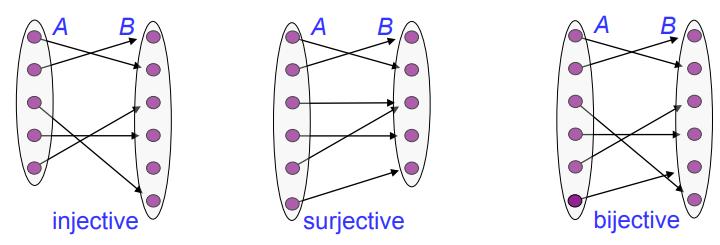
\includegraphics[scale=0.7]{types}
\end{center}
\section{More on bijections}
\begin{itemize}
	\item Suppose that $f: A\rightarrow B$ is a bijection
	\item We can build a set of ordered pairs
	$$P = \{ ( a , f ( a ) ) : a \in A \} \subseteq A \times B$$
	\item As f is onto every $b\in B$ must appear as the second component in some pair (a,b)
	\item As f is one-to-one every $b\in B$ must appear as the second component in at most one pair (a,b)
	\item So, each element of A appears in exactly one pair in P, as does each element of B
	\item The set P is a "pairing" of the elements of A and B so that every element of A is associated with a unique element of B, and vice versa
\end{itemize}
\section{Compositions of functions}
Suppose that $f: A\rightarrow B$ and $g: B\Rightarrow C$ are functions. We can define the composition of g and f as the function $g \circ f : A \rightarrow C$ defined as $( g \circ f ) ( x ) = g ( f ( x ) )$\\
\\
Note that even if the function $g\circ f$ exists, the function $f\circ g$ might not exist\\
\\
Also, even if both $g\circ f$ and $f\circ g$ exist, it could well be that they are different
\section{Inverses}
Often we want the inverse of a function, where the inverse of the function $f: A\rightarrow B$ is the function $f^{-1}: B\rightarrow A$ where:
\begin{itemize}
	\item $f ^ { - 1 } ( f ( a ) ) = a , \forall a \in A$
	\item $f \left( f ^ { - 1 } ( b ) \right) = b , \forall b \in B$
\end{itemize}
\begin{center}
	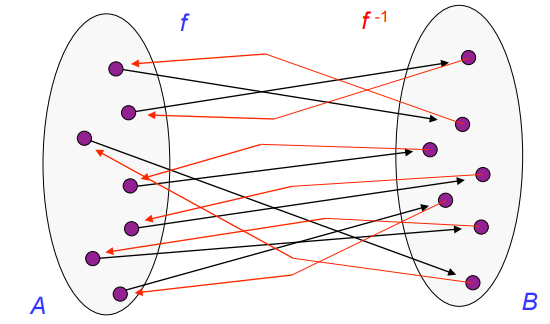
\includegraphics[scale=0.7]{inverse}
\end{center}
\begin{itemize}
	\item Note that it may not always be the case that the inverse function exists
	\item Let $f: A\rightarrow B$
	\begin{itemize}
		\item Suppose that f is not one to one, i.e. $\exists$ distinct $a , a ^ { \prime } \in A \text { s.t. } f ( a ) = f \left( a ^ { \prime } \right)$
		\item If $f^{-1}$ exists then $a = f ^ { - 1 } ( f ( a ) ) = f ^ { - 1 } \left( f \left( a ^ { \prime } \right) \right) = a ^ { \prime }$ which yields a contradiction
		\item So, if an inverse of f exists then f must be one to one
		\item Suppose that f is not onto, i.e. $\exists b\in B$ s.t. there is not $a\in A$ s.t. $f(a)=b$
		\item If $f^{-1}$ exists then $f^{-1}(b)=a'$ for some $a'\in A$ with $b = f \left( f ^ { - 1 } ( b ) \right) = f \left( a ^ { \prime } \right)$, which yields a contradiction
		\item So, if an inverse of f exists then f must be onto
		\item So, if an inverse of f exists then f must be a bijection
		\item Conversely, if f is one-to-one and onto then the inverse exists. We simply define $f^{-1}(b)$ as the unique element $ain A$ for which $f(a)=b$. Since f is a bijection, we can "pair" elements of A and B so that each element of A is associates with a unique element of B, and vice versa
	\end{itemize}
	\item This, we have proven that f has an inverse if, and only if, f is a bijection
\end{itemize}
\section{Cardinality Revisited}
\begin{itemize}
	\item Two sets A and B (which may be finite or infinite) have the same cardinality iff there is a bijection from A to B
	\item A set is countable if it is finite or has the same cardinality as N when we say it has cardinality $\aleph_0$
	\item A set is uncountable if it does not have cardinality $\aleph_0$
\end{itemize}
\section{Uncountable sets}
\begin{itemize}
	\item Up until not, we have not even shown that there exist uncountable sets, however these sets do exist and $\mathbb{R}$ is one of them
	\item Suppose that R is countable
	\begin{itemize}
		\item This the set I of real number strictly between 0 and 1 is countable, that is, there is a bijection $f:\mathbb{N}\rightarrow I$
		\item List all the elements of $\mathbb{R}$
		\item "pull out" those between 0 and 1 and put them in a sub-list
	\end{itemize}
	\item Form a new decimal number x between 0 and 1 by building the number whose ith digit behind the decimal point is 5 ith the ith digit of f(i-1) is 4 and 4 otherwise
	\item By definition x is not equal to any number on the list
	\begin{itemize}
		\item its ith digit of x behind the decimal point is different from the ith digit behind the decimal point of the ith number in the list
		\item So f is not onto, which yields a contradiction
	\end{itemize}
	\item Thus, $\mathbb{R}$ is uncountable and has cardinality "bigger" that $\aleph_0$
	\item The generic technique employed is called \textbf{diagonalization}
\end{itemize}

\end{document}